\documentclass[12pt, twoside]{book}
%\documentclass[12pt, oneside]{book}  % jednostranna tlac

%spravne nastavenie okrajov
\usepackage[a4paper,top=2.5cm,bottom=2.5cm,left=3.5cm,right=2cm]{geometry}
\usepackage{amsmath,amssymb}
\usepackage{array}

%zapnutie fontov pre UTF8 kodovanie
\usepackage[utf8]{inputenc}
\usepackage[T1]{fontenc}

%zapnutie slovenskeho delenia slov
%a automatickych nadpisov ako Obsah, Obrázok a pod. v slovencine
%\usepackage[slovak]{babel} % vypnite pre prace v anglictine!
\usepackage[english]{babel}

%nastavenie riadkovania podla smernice
\linespread{1.25} % hodnota 1.25 by mala zodpovedat 1.5 riadkovaniu

% balicek na vkladanie zdrojoveho kodu
\usepackage{listings}
% ukazky kodu su cislovane ako Listing 1,2,...
% tu je Listing zmenene na Algoritmus 1,2,...
% \renewcommand{\lstlistingname}{Algorithm}
% nastavenia balicka listings
% mozete pridat aj language=...
% na nastavenie najcastejsie pouzivaneho prog. jazyka
% takisto sa da zapnut cislovanie riadkov
\lstset{frame=lines}

% balicek na vkladanie obrazkov
\usepackage{graphicx}
% balicek na vkladanie celych pdf dokumentov, tu zadanie
\usepackage{pdfpages}
% balicek na spravne formatovanie URL
\usepackage{url}
% balicek na hyperlinky v ramci dokumentu
% zrusime farebne ramiky okolo liniek aby pdf
% vyzeralo rovnako ako tlacena verzia
\usepackage[hidelinks,breaklinks]{hyperref}


% -------------------
% --- Definicia zakladnych pojmov
% --- Vyplnte podla vasho zadania, rok ma byt rok odovzdania
% -------------------
\def\mfrok{2026}
\def\mfnazov{Classical Knapsack Cryptosystem and its variations}
\def\mftyp{Bachelor Thesis}
\def\mfautor{David Vavřinek}
\def\mfskolitel{doc. RNDr. Tatiana Jajcayová, PhD.}

%ak mate konzultanta, odkomentujte aj jeho meno na titulnom liste
\def\mfkonzultant{tit. Meno Priezvisko, tit. }  

\def\mfmiesto{Bratislava, \mfrok}

% študenti BIN a DAV odkomentujú príslušnú dvojicu riadkov
\def\mfodbor{Computer Science}               % Field of Study (official Slovak)
\def\program{Applied Computer Science}  % Study Programme (English)
% Ak máte externého školiteľa, uvádzajte Katedru informatiky 
\def\mfpracovisko{Department of Applied Informatics}

\begin{document}     
\frontmatter
\pagestyle{empty}

% -------------------
% --- Obalka ------
% -------------------

\begin{center}
  \sc\large
  Comenius University in Bratislava\\
  Faculty of Mathematics, Physics and Informatics

\vfill

{\LARGE\mfnazov}\\
\mftyp
\end{center}

\vfill

{\sc\large 
\noindent \mfrok\\
\mfautor
}

\cleardoublepage
% --- koniec obalky ----

% -------------------
% --- Titulný list
% -------------------

\noindent

\begin{center}
\sc  
\large
  Comenius University in Bratislava\\
  Faculty of Mathematics, Physics and Informatics

\vfill

{\LARGE\mfnazov}\\
\mftyp
\end{center}

\vfill

\noindent
\begin{tabular}{ll}
Study Programme: & \program \\
Field of Study: & \mfodbor \\
Department: & \mfpracovisko \\
Supervisor: & \mfskolitel \\
% Consultant: & \mfkonzultant \\
\end{tabular}

\vfill


\noindent \mfmiesto\\
\mfautor

\cleardoublepage
% --- Koniec titulnej strany


% -------------------
% --- Zadanie z AIS
% -------------------
% v tlačenej verzii s podpismi zainteresovaných osôb.
% v elektronickej verzii sa zverejňuje zadanie bez podpisov
% v pracach v anglictine anglicke aj slovenske zadanie

\newpage
\setcounter{page}{2}
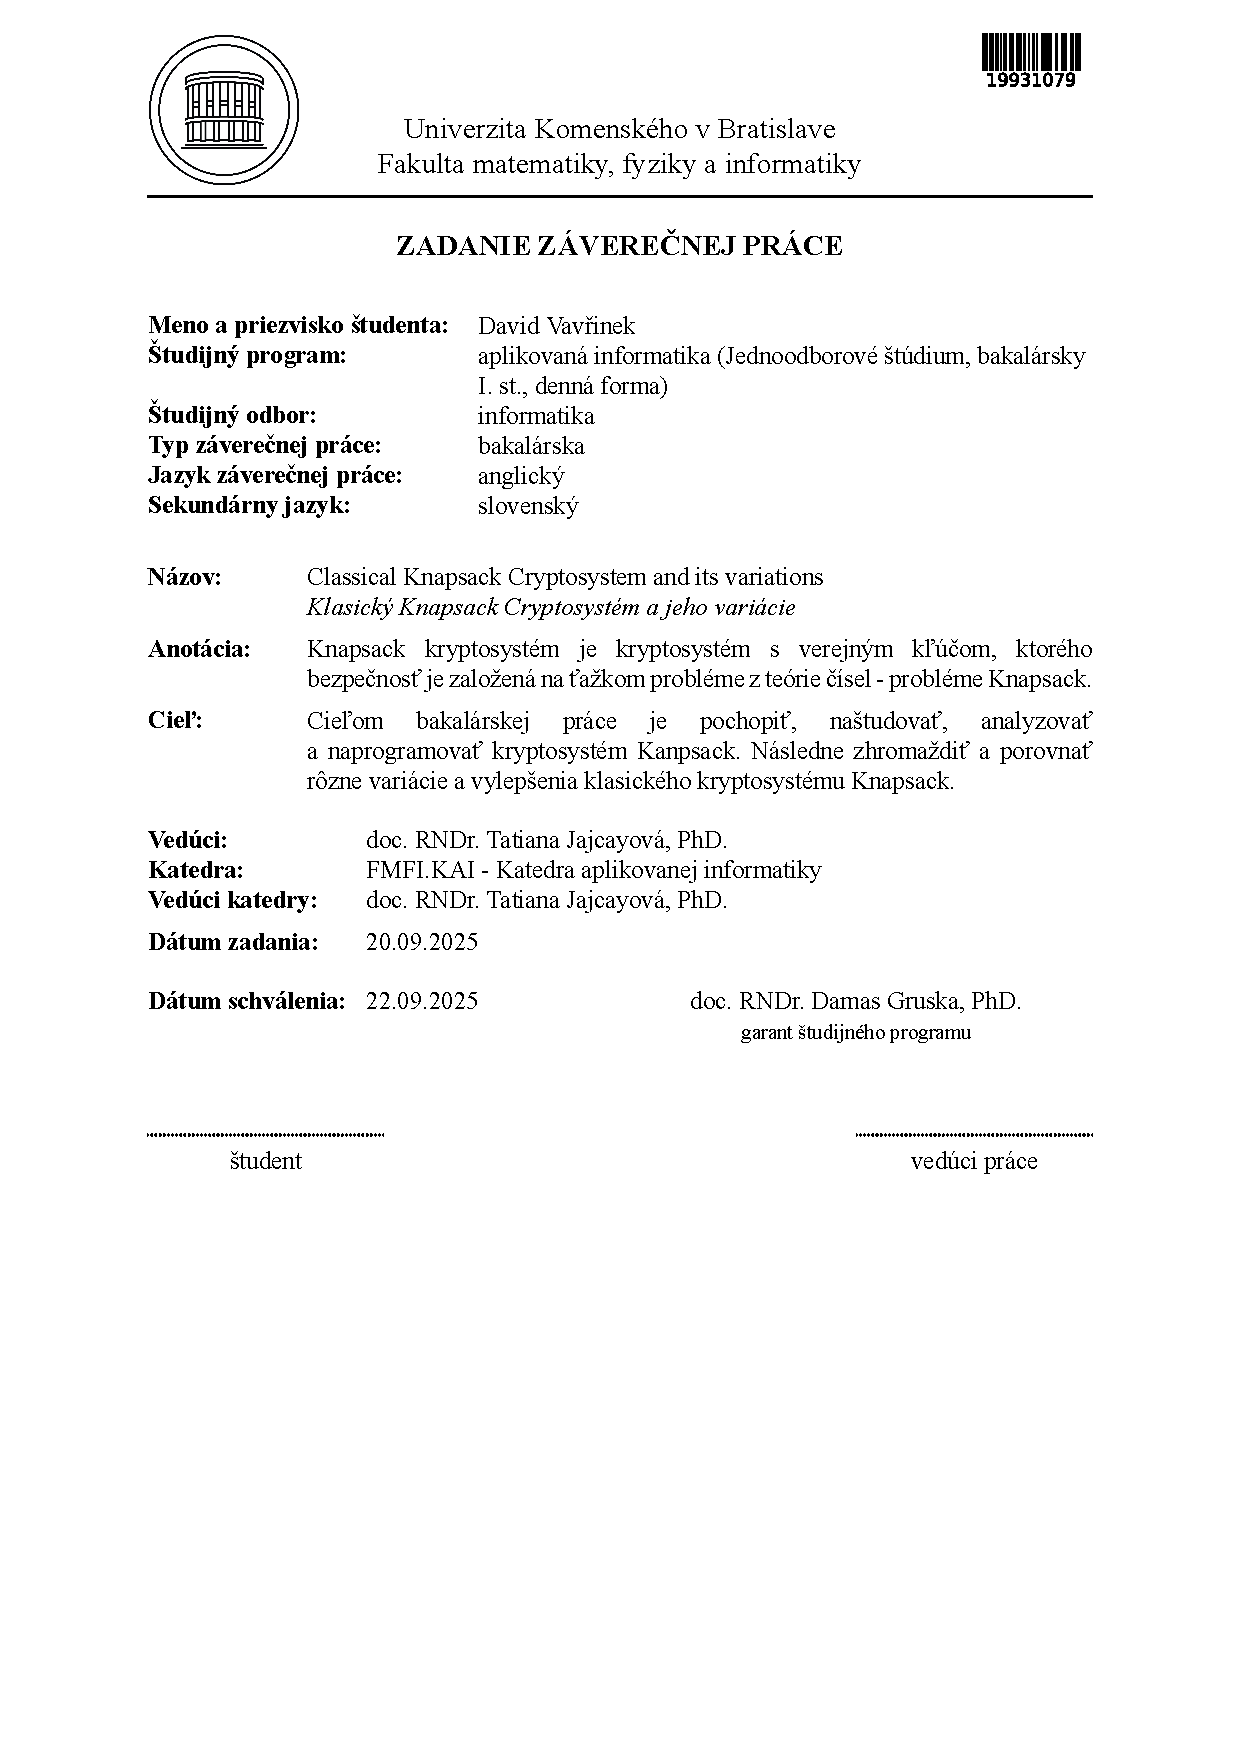
\includepdf{images/zadanie.pdf}

\includepdf{images/zadanie-en.pdf}

% --- Koniec zadania

\newpage
\chapter*{Declaration}

I hereby declare that I prepared this bachelor thesis independently and used
only the literature and sources listed in the bibliography.

During the preparation of the thesis, I used artificial intelligence tools as
supporting tools, mainly for language correction, stylistic suggestions,
structural feedback, LaTeX assistance, and help with checking and debugging the
implementation. The tools were not used as a substitute for my own work. I
checked their outputs and I am responsible for the final text, implementation,
experiments, and conclusions.

% -------------------
%   Poďakovanie - nepovinné
% -------------------
\newpage
\pagestyle{plain}
~

\vfill
{\bf Acknowledgments:} I would like to thank my supervisor doc. RNDr. Tatiana Jajcayová, PhD.,
for her guidance, consultations, and helpful comments during the preparation of
this bachelor thesis.

% --- Koniec poďakovania

% -------------------
% --- Abstract - English
% -------------------
\newpage 
\chapter*{Abstract}

Knapsack cryptosystems were among the first attempts to build public-key
cryptography from the subset-sum problem. This idea was attractive because the
decision version of subset-sum is NP-complete. The later history of these
systems, showed that this argument is not sufficient for security. The
public-key instances generated by a cryptosystem may contain hidden
structure that an attacker can exploit.

This thesis examines this problem through the classical Merkle--Hellman
knapsack cryptosystem and several related variants. It explains how the
superincreasing trapdoor works, why the basic construction is vulnerable to
Shamir's polynomial-time attack, and how lattice methods affect low-density
knapsack instances and later modifications. The practical part implements the
classical, permuted, and simple iterated variants in C. The experiments verify
the implementation, compare the runtime of the variants, and show how selected
parameters influence the density of the public knapsack. The main conclusion is
that classical knapsack cryptosystems are no longer suitable for practical
public-key encryption, but they remain useful as a historical and educational
example. They show that the theoretical hardness of a problem does not by
itself guarantee the security of a concrete cryptographic construction.

\paragraph*{Keywords:} knapsack cryptosystem, subset-sum, Merkle--Hellman, cryptanalysis
% --- End Abstract - English


% -------------------
% --- Predhovor - v informatike sa zvacsa nepouziva
% -------------------
%\newpage 
%
%
%\chapter*{Preface} %
%
%Predhovor je všeobecná informácia o práci, obsahuje hlavnú charakteristiku práce 
%a okolnosti jej vzniku. Autor zdôvodní výber témy, stručne informuje o cieľoch 
%a význame práce, spomenie domáci a zahraničný kontext, komu je práca určená, 
%použité metódy, stav poznania; autor stručne charakterizuje svoj prístup a svoje
%hľadisko. 
%
% --- Koniec Predhovor


% -------------------
% --- Obsah
% -------------------

\newpage 

\tableofcontents

% ---  Koniec Obsahu

% -------------------
% --- Zoznamy tabuliek, obrázkov - nepovinne
% -------------------

\newpage 

\listoffigures
\listoftables

% ---  Koniec Zoznamov

\mainmatter
\pagestyle{headings}

\input introduction.tex 

\input theory.tex
\input variations.tex
\input implementation.tex
\input results.tex
\input conclusion.tex


% \chapter{A Sample Text}
% Chapters in Slovak language are commented out, but use them as a guide
% to write chapters in English. Here we only cite some references, such
% as a book about LaTeX \cite{Oetiker2000}, a scientific journal article
% \cite{clanok}, a conference paper \cite{clanok_na_konferencii}, a
% technical report \cite{technical_report}, a book \cite{kniha}, and a
% resource from the Internet \cite{smernica}.


%\input zaver.tex

% -------------------
% --- Bibliografia
% -------------------


\newpage	

\backmatter

\thispagestyle{empty}
\clearpage

\bibliographystyle{plain}
\bibliography{literatura} 

%Prípadne môžete napísať literatúru priamo tu
%\begin{thebibliography}{5}
 
%\bibitem{br1} MOLINA H. G. - ULLMAN J. D. - WIDOM J., 2002, Database Systems, Upper Saddle River : Prentice-Hall, 2002, 1119 s., Pearson International edition, 0-13-098043-9

%\bibitem{br2} MOLINA H. G. - ULLMAN J. D. - WIDOM J., 2000 , Databasse System implementation, New Jersey : Prentice-Hall, 2000, 653s., ???

%\bibitem{br3} ULLMAN J. D. - WIDOM J., 1997, A First Course in Database Systems, New Jersey : Prentice-Hall, 1997, 470s., 

%\bibitem{br4} PREFUSE, 2007, The Prefuse visualization toolkit,  [online] Dostupné na internete: <http://prefuse.org/>

%\bibitem{br5} PREFUSE Forum, Sourceforge - Prefuse Forum,  [online] Dostupné na internete: <http://sourceforge.net/projects/prefuse/>

%\end{thebibliography}

%---koniec Referencii

% -------------------
%--- Prilohy---
% -------------------

%Nepovinná časť prílohy obsahuje materiály, ktoré neboli zaradené priamo  do textu. Každá príloha sa začína na novej strane.
%Zoznam príloh je súčasťou obsahu.
%
%\input appendixA.tex

%\input appendixB.tex

\end{document}






